\section{Resultados}

\begin{enumerate}
	\item Las inconsistencias fueron visualizadas fácilmente debido a los saltos que existían entre los clientes que tenían una latencia simulada mayor a 0. Es posible ver la trayectoria original de los objetos gracias a la renderización sobre estados anteriores del juego.
	\item Se puede percibir el efecto del \emph{local-lag}. Si es muy alto, existe mayor consistencia pero menor responsividad; si es moderado se ve que la sincronización es estable y si es muy bajo se visualizan las inconsistencias como se describe en 1.
\end{enumerate}

En términos generales se puede comprobar la teoría con la implementación de los protocolos con las distintas variables en juego que pueden ser simuladas a discreción.


\begin{figure}[h]
\centering
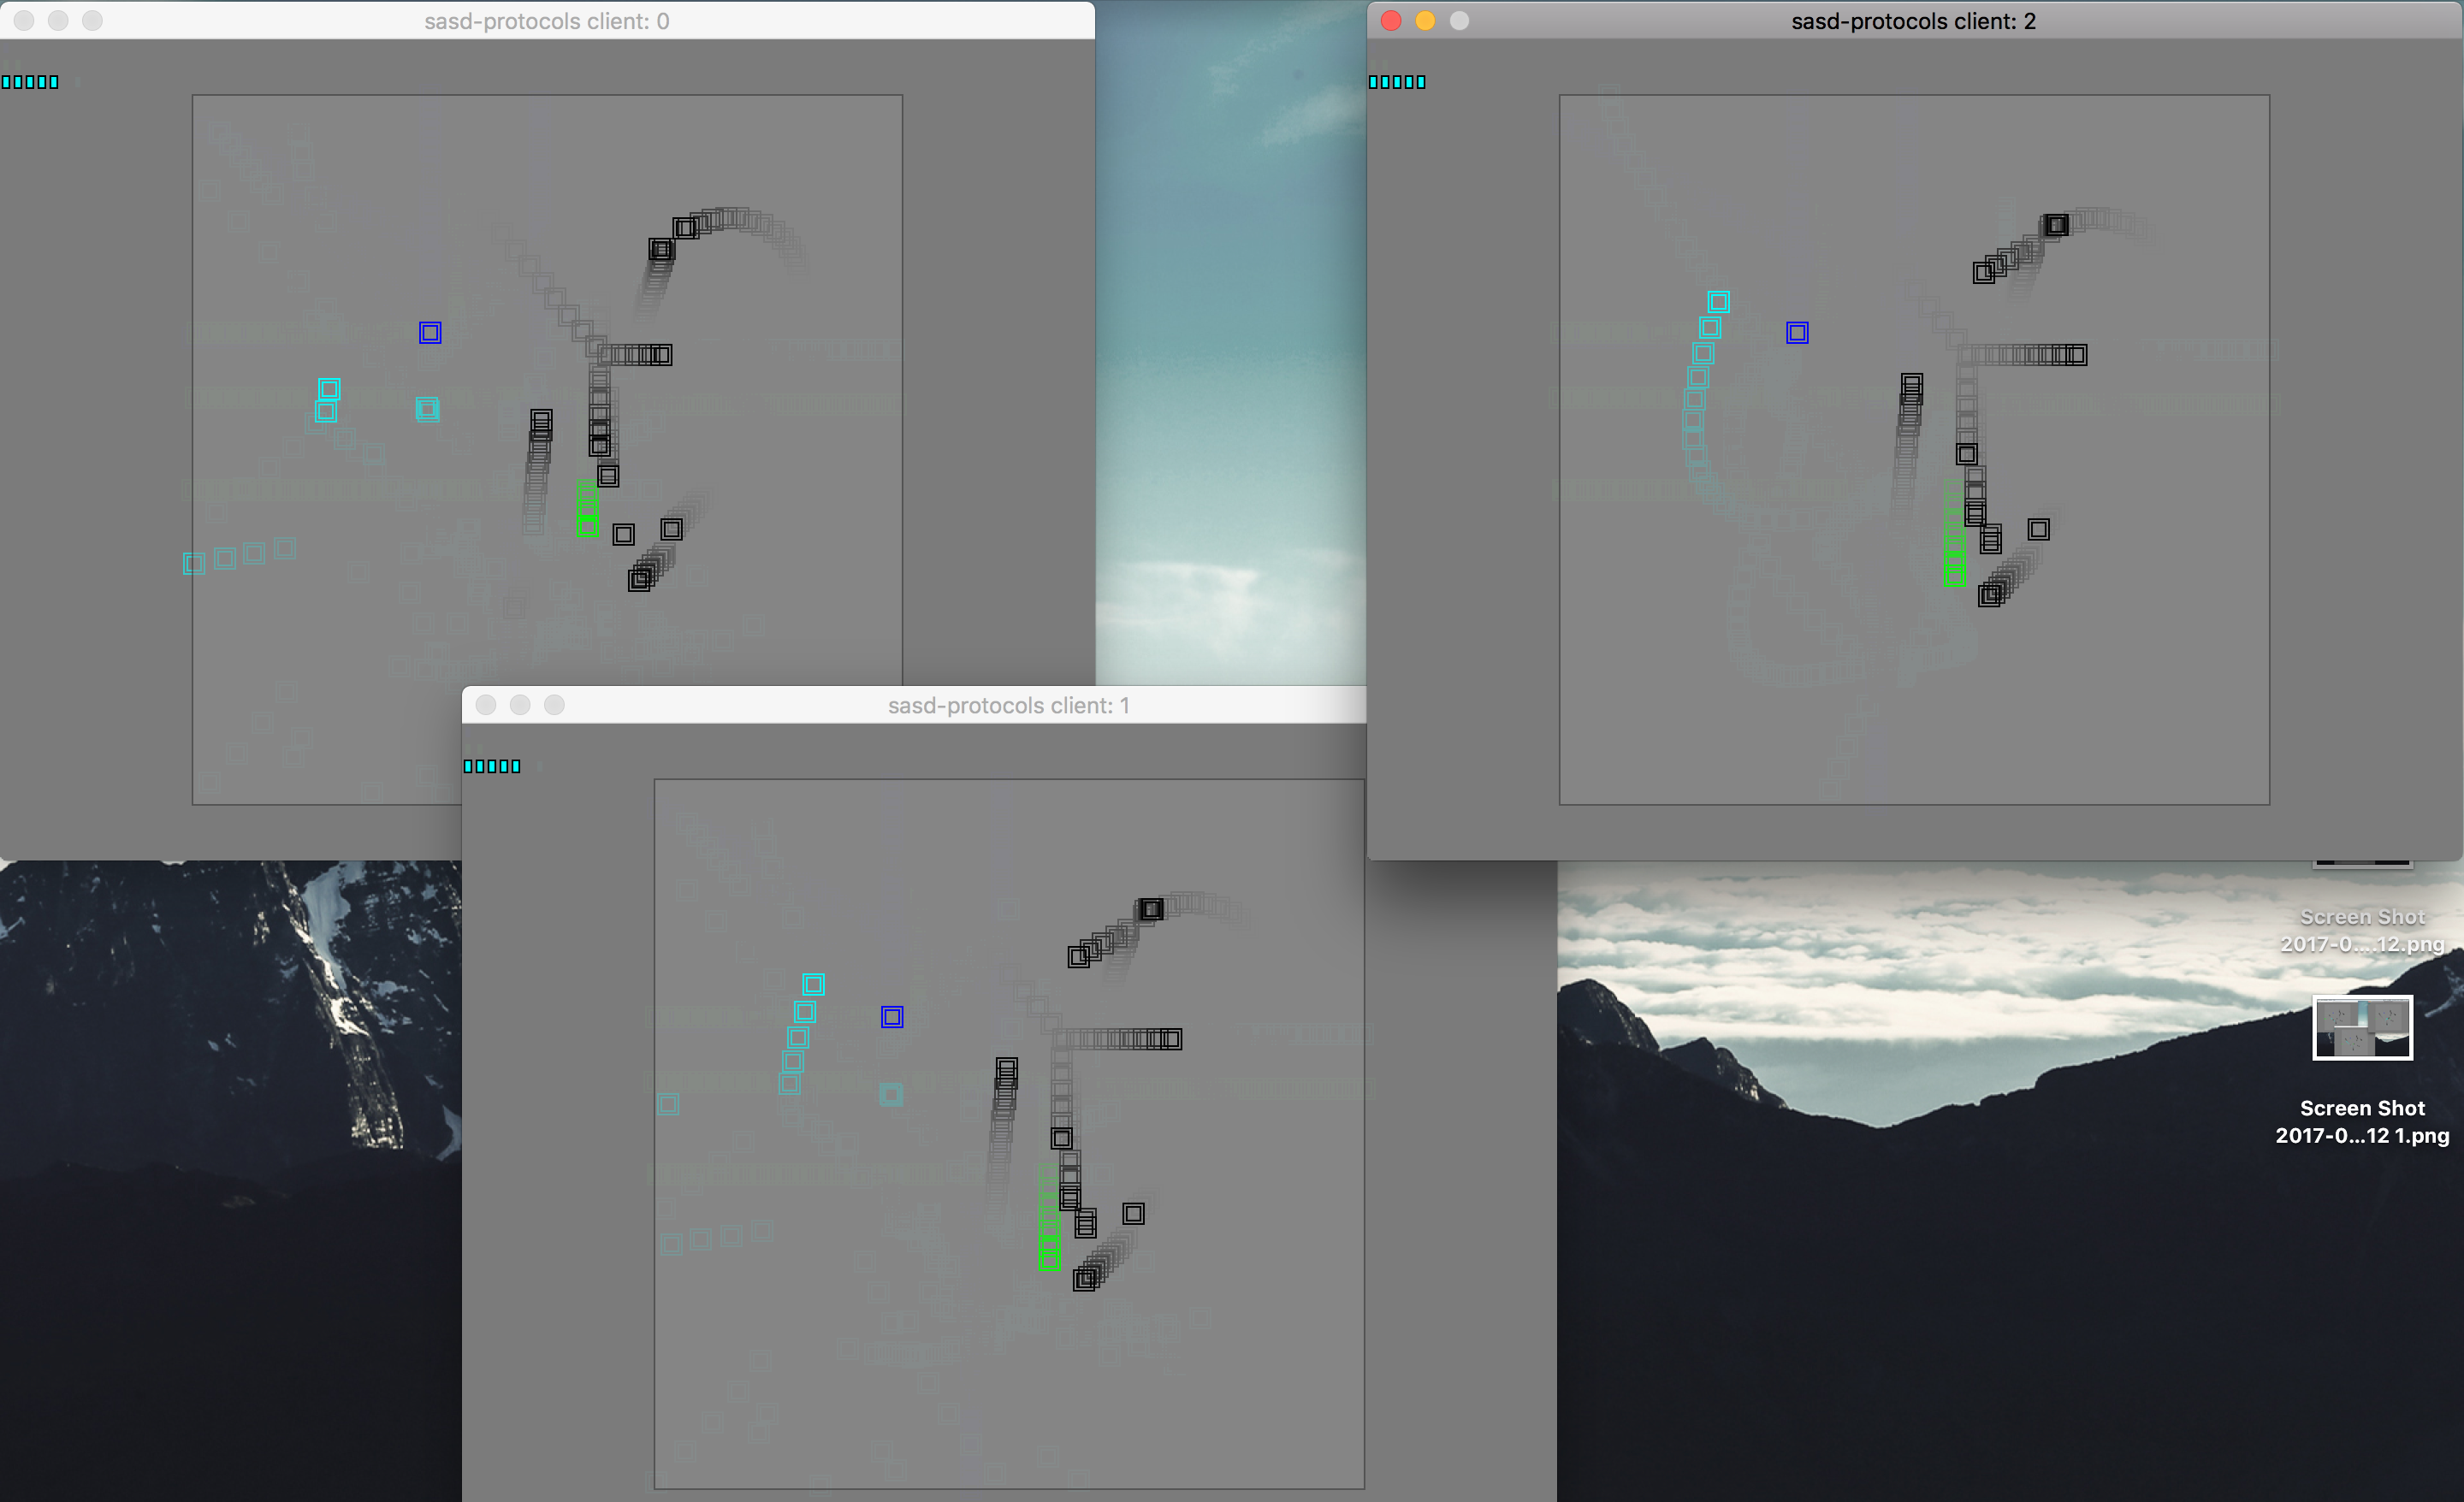
\includegraphics[width=0.8\textwidth]{run}
\caption{\label{fig:execution} \small Ejecución de varios clientes conectados corriendo en una misma máquina con el protocolo \emph{Timewarp} implementado en el \emph{framework}.} Se simuló una gran latencia entre los clientes, se puede ver que el cliente $2$ (color celeste) se movió hacia arriba y los otros tuvieron que aplicar \emph{rollbacks}, lo que se vio como un salto. Mientras que los clientes 0 y 1 están relativamente sincronizados.
\end{figure}


% Identificar cualitativamente los resultados del retraso de la red en cada uno de los métodos.
